\section{A Hardware-Efficient Algorithm for SSD Models}
\label{sec:efficient}


The benefits of developing the theoretical SSD framework between SSMs, attention, and structured matrices lies in using the connections to improve the models and algorithms.
In this section, we show how various algorithms for computing SSD models efficiently can be derived from various algorithms for computing structured matrix multiplication.

\iftoggle{arxiv}{
Our main computational result is an algorithm for computing SSD models that combines both the linear (recurrent) mode and quadratic (attention) mode.
This algorithm is as computation efficient as SSMs (linear scaling in sequence length) and as hardware-friendly as attention (primarily uses matrix multiplications).


\begin{theorem}
  \label{thm:algorithm}
  Consider an SSD model with state expansion factor $\mathtt{N}$ and head dimension $\mathtt{P}=\mathtt{N}$.
  There exists an algorithm for computing the model on any input $X \in \R^{\mathtt{(T, P)}}$
  which only requires $O(\mathtt{TN}^2)$ training FLOPs, $O(\mathtt{TN})$ inference FLOPs,
  $O(\mathtt{N}^2)$ inference memory,
  and whose work is dominated by matrix multiplications.
\end{theorem}
Note that all of these bounds are tight, because
a state space model with state expansion $\mathtt{N}$ operating on a head size of $\mathtt{N}$ has total state size $\mathtt{N}^2$ (yielding the lower bounds for training and inference FLOPs of $O(\mathtt{TN}^2)$ and $O(\mathtt{N}^2)$ respectively).
Furthermore the input $X$ itself has $\mathtt{TN}$ elements, yielding the memory lower bound.

The main idea behind \cref{thm:algorithm} is once again viewing the problem of computing a state space model as a semiseparable matrix multiplication, but leveraging its structure in a new way.
Instead of computing the whole matrix in either recurrent or attention mode,
we perform a \emph{block decomposition} of the matrix.
The diagonal blocks can be computed using the dual attention mode, which can be efficiently done with matrix multiplications,
while the off-diagonal blocks can be factored by the rank-structure of semiseparable matrices and reduced to a smaller recurrence.
We highlight that \cref{listing} provides a self-contained implementation of the SSD algorithm.
Compared to the general selective SSM of \citet{gu2023mamba},
this implementation is much simpler, and relatively efficient even in native PyTorch without requiring special low-level kernels.
}{
}




To begin, we partition the matrix $M$ into a $\frac{\mathtt{T}}{\mathtt{Q}} \times \frac{\mathtt{T}}{\mathtt{Q}}$ grid of submatrices of size $\mathtt{Q} \times \mathtt{Q}$,
for some block size $\mathtt{Q}$.
Note that the off-diagonal blocks are low-rank by the defining property of semiseparable matrices (\cref{def:semiseparable-rank}).%
\footnote{Note that the block decomposition is valid even with partitions of varying size, e.g.\ if $\mathtt{Q} \not\mid \mathtt{T}$, but we assume even divisibility for simplicity.}
\begin{align*}%
  \text{(Block Decomposition)} \quad M &=
  \begin{bmatrix}
    M^{(0,0)} \\
    M^{(1,0)} & M^{(1,1)} \\
    \vdots & \vdots & \ddots \\
    M^{(\mathtt{T}/\mathtt{Q}-1,0)} & M^{(\mathtt{T}/\mathtt{Q}-1,1)} & \dots & M^{(\mathtt{T}/\mathtt{Q}-1,\mathtt{T}/\mathtt{Q}-1)} \\
  \end{bmatrix}
  \\
  \text{(Diagonal Block)} \quad M^{(j,j)} &= \mathsf{SSM}(A_{j\mathtt{Q}:(j+1)\mathtt{Q}}, B_{j\mathtt{Q}:(j+1)\mathtt{Q}}, C_{j\mathtt{Q}:(j+1)\mathtt{Q}}) \\
  \text{(Low-Rank Block)} \quad M^{(j,i)} &= 
  \begin{bmatrix}C_{j\mathtt{Q}}^{\top} A_{j\mathtt{Q}:j\mathtt{Q}-1} \\[1pt] \vdots \\[1pt] C_{(j+1)\mathtt{Q}-1}^{\top} A_{(j+1)\mathtt{Q}-1:j\mathtt{Q}-1}\end{bmatrix}
  A_{j\mathtt{Q}-1:(i+1)\mathtt{Q}-1}
  \begin{bmatrix}B_{i\mathtt{Q}}^{\top} A_{(i+1)\mathtt{Q}-1:i\mathtt{Q}} \\[1pt] \vdots \\[1pt] B_{(i+1)\mathtt{Q}-1}^{\top} A_{(i+1)\mathtt{Q}-1:(i+1)\mathtt{Q}-1}\end{bmatrix}^{\top}
\end{align*}

This is easiest illustrated through an example, e.g.\ for $\mathtt{T}=9$ and decomposing into chunks of length $\mathtt{Q}=3$.
The shaded cells are low-rank factorizations of the off-diagonal blocks of the semiseparable matrix.
\begin{align*}%
M &=
\begin{bNiceArray}{ccc|ccc|ccc}[cell-space-limits=2pt]
    C_0^{\top} A_{0:0} B_0 & \\
    C_1^{\top} A_{1:0} B_0 & C_1^{\top} A_{1:1} B_1 & \\
    C_2^{\top} A_{2:0} B_0 & C_2^{\top} A_{2:1} B_1 & C_2^{\top} A_{2:2} B_2 \\
    \hline
    C_3^{\top} A_{3:0} B_0 & C_3^{\top} A_{3:1} B_1 & C_3^{\top} A_{3:2} B_2 & C_3^{\top} A_{3:3} B_3 \\
    C_4^{\top} A_{4:0} B_0 & C_4^{\top} A_{4:1} B_1 & C_4^{\top} A_{4:2} B_2 & C_4^{\top} A_{4:3} B_3 & C_4^{\top} A_{4:4} B_4 \\
    C_5^{\top} A_{5:0} B_0 & C_5^{\top} A_{5:1} B_1 & C_5^{\top} A_{5:2} B_2 & C_5^{\top} A_{5:3} B_3 & C_5^{\top} A_{5:4} B_4 & C_5^{\top} A_{5:5} B_5 \\
    \hline
    C_6^{\top} A_{6:0} B_0 & C_6^{\top} A_{6:1} B_1 & C_6^{\top} A_{6:2} B_2 & C_6^{\top} A_{6:3} B_3 & C_6^{\top} A_{6:4} B_4 & C_6^{\top} A_{6:5} B_5 & C_6^{\top} A_{6:6} B_6 \\
    C_7^{\top} A_{7:0} B_0 & C_7^{\top} A_{7:1} B_1 & C_7^{\top} A_{7:2} B_2 & C_7^{\top} A_{7:3} B_3 & C_7^{\top} A_{7:4} B_4 & C_7^{\top} A_{7:5} B_5 & C_7^{\top} A_{7:6} B_6 & C_7^{\top} A_{7:7} B_7 \\
    C_8^{\top} A_{8:0} B_0 & C_8^{\top} A_{8:1} B_1 & C_8^{\top} A_{8:2} B_2 & C_8^{\top} A_{8:3} B_3 & C_8^{\top} A_{8:4} B_4 & C_8^{\top} A_{8:5} B_5 & C_8^{\top} A_{8:6} B_6 & C_8^{\top} A_{8:7} B_7 & C_8^{\top} A_{8:8} B_8 \\
\end{bNiceArray}
\\
\\&=
\begin{bNiceArray}{ccc|ccc|ccc}[cell-space-limits=2pt]
    C_0^{\top} A_{0:0} B_0 & \\
    C_1^{\top} A_{1:0} B_0 & C_1^{\top} A_{1:1} B_1 & \\
    C_2^{\top} A_{2:0} B_0 & C_2^{\top} A_{2:1} B_1 & C_2^{\top} A_{2:2} B_2 \\
    \hline
    \Block[fill=[RGB]{243,240,255}]{3-3}{\begin{bmatrix}C_3^{\top} A_{3:2} \\[1pt] C_4^{\top} A_{4:2} \\[1pt] C_5^{\top} A_{5:2}\end{bmatrix}A_{2:2}\begin{bmatrix}B_0^{\top} A_{2:0} \\[1pt] B_1^{\top} A_{2:1} \\[1pt] B_2^{\top} A_{2:2}\end{bmatrix}^{\top}}
                           &&& C_3^{\top} A_{3:3} B_3 \\
                           &&& C_4^{\top} A_{4:3} B_3 & C_4^{\top} A_{4:4} B_4 \\
                           &&& C_5^{\top} A_{5:3} B_3 & C_5^{\top} A_{5:4} B_4 & C_5^{\top} A_{5:5} B_5 \\
    \hline
    \Block[fill=[RGB]{243,240,255}]{3-3}{\begin{bmatrix}C_6^{\top} A_{6:5} \\[1pt] C_7^{\top} A_{7:5} \\[1pt] C_8^{\top} A_{8:5}\end{bmatrix}A_{5:2}\begin{bmatrix}B_0^{\top} A_{2:0} \\[1pt] B_1^{\top}A_{2:1} \\[1pt] B_2^{\top}A_{2:2}\end{bmatrix}^{\top}}
                           &&&
                           \Block[fill=[RGB]{243,240,255}]{3-3}{\begin{bmatrix}C_6^{\top} A_{6:5} \\[1pt] C_7^{\top} A_{7:5} \\[1pt] C_8^{\top} A_{8:5}\end{bmatrix}A_{5:5}\begin{bmatrix}B_3^{\top}A_{5:3} \\[1pt] B_4^{\top}A_{5:4} \\[1pt] B_5^{\top}A_{5:5}\end{bmatrix}^{\top}}
                           &&& C_6^{\top} A_{6:6} B_6 \\
                           &&&&&& C_7^{\top} A_{7:6} B_6 & C_7^{\top} A_{7:7} B_7 \\
                           &&&&&& C_8^{\top} A_{8:6} B_6 & C_8^{\top} A_{8:7} B_7 & C_8^{\top} A_{8:8} B_8 \\
  \end{bNiceArray}
\end{align*}

From here we can reduce the problem into these two parts.
These can also be interpreted as dividing the output of a ``chunk'' $y_{j\mathtt{Q}:(j+1)\mathtt{Q}}$ into two components:
the effect of inputs within the chunk $x_{j\mathtt{Q}:(j+1)\mathtt{Q}}$, and the effect of inputs before the chunk $x_{0:j\mathtt{Q}}$.

\subsection{Diagonal Blocks}
The diagonal blocks are easy to handle, because they are simply self-similar problems of a smaller size.
The $j$-th block represents computing the answer $\mathsf{SSM}(A_R, B_R, C_R)(x_R)$ for the range $R = j\mathtt{Q}:(j+1)\mathtt{Q} = (j\mathtt{Q}, j\mathtt{Q}+1, \dots, j\mathtt{Q}+\mathtt{Q}-1)$.
The key is that this block can be computed using any desired method.
In particular, for small chunk lengths $\mathtt{Q}$, this problem is computed more efficiently using the dual quadratic SMA form.
Additionally, the chunks can be computed in parallel.

These subproblems can be interpreted as: what is the output per chunk \emph{supposing that the initial state (to the chunk) is $0$}.
In other words for chunk $j$, this computes the correct outputs taking into account only the chunk inputs $x_{j\mathtt{Q}:(j+1)\mathtt{Q}}$.

\subsection{Low-Rank Blocks}

The low-rank factorizations consist of 3 terms, and there are correspondingly three pieces of the computation.
In this factorization, we will use the terminology
\begin{itemize}
  \item The terms like $\begin{bmatrix}B_0^{\top} A_{2:0} \\[1pt] B_1^{\top}A_{2:1} \\[1pt] B_2^{\top}A_{2:2}\end{bmatrix}^{\top}$ are called the right factors or $B$-block-factors.
  \item The terms like $A_{5:2}$ are called the center factors or $A$-block-factors.
  \item The terms like $\begin{bmatrix}C_6^{\top} A_{6:5} \\[1pt] C_7^{\top} A_{7:5} \\[1pt] C_8^{\top} A_{8:5}\end{bmatrix}$ are called the left factors or $C$-block-factors.
\end{itemize}


\paragraph{Right Factors.}

This step computes the multiplication by the right $B$-block-factors of the low-rank factorization.
Note that for each chunk, this is a $(\mathtt{N}, \mathtt{Q})$ by $(\mathtt{Q}, \mathtt{P})$ matrix multiplication, where $\mathtt{N}$ is the state dimension and $P$ is the head dimension.
The result is a $(\mathtt{N}, \mathtt{P})$ tensor for each chunk, which has the same dimensionality as the expanded hidden state $h$.

This can be interpreted as: what is the final state per chunk \emph{supposing that the initial state (to the chunk) is $0$}.
In other words this computes $h_{j\mathtt{Q}+\mathtt{Q}-1}$ assuming that $x_{0:j\mathtt{Q}} = 0$.

\paragraph{Center Factors.}

This step computes the effect of the center $A$-block-factors terms in the low-rank factorization.
In the previous step, the final states per chunk have total shape $\mathtt{(\mathtt{T}/\mathtt{Q},\mathtt{N},\mathtt{P})}$.
This is now multiplied by a 1-SS matrix generated by $A_{2\mathtt{Q}-1:\mathtt{Q}-1}^\times, A_{3\mathtt{Q}-1:2\mathtt{Q}-1}^\times, \dots, A_{\mathtt{T}-1:\mathtt{T}-\mathtt{Q}-1}^\times$.

This step can be computed by any algorithm for computing 1-SS multiplication (also known as the scalar SSM scan or \texttt{cumprodsum} operator).

This can be interpreted as: what is the actual final state per chunk \emph{taking into account all previous inputs};
in other words, this computes the true hidden state $h_{j\mathtt{Q}}$ taking into account all of $x_{0:(j+1)\mathtt{Q}}$.

\paragraph{Left Factors.}

This step computes the multiplication by the left $C$-block-factors of the low-rank factorization.
For each chunk, this can be represented by a matrix multiplication
$\mathsf{contract}(\mathtt{QN,NP \to QP})$.

This can be interpreted as: what is the output per chunk \emph{taking into account the correct initial state $h_{j\mathtt{Q}-1}$, and supposing the inputs $x_{j\mathtt{Q}:(j+1)\mathtt{Q}}$ are $0$}.
In other words for chunk $j$, this computes the correct outputs taking into account only the prior inputs $x_{0:j\mathtt{Q}}$.

\begin{listing*}[!t]
\inputminted[fontsize=\footnotesize]{python}{structure/code.py}
\caption{Full PyTorch example of the state space dual (SSD) model.}
\label{listing}
\end{listing*}


\begin{figure}[!t]
\centering
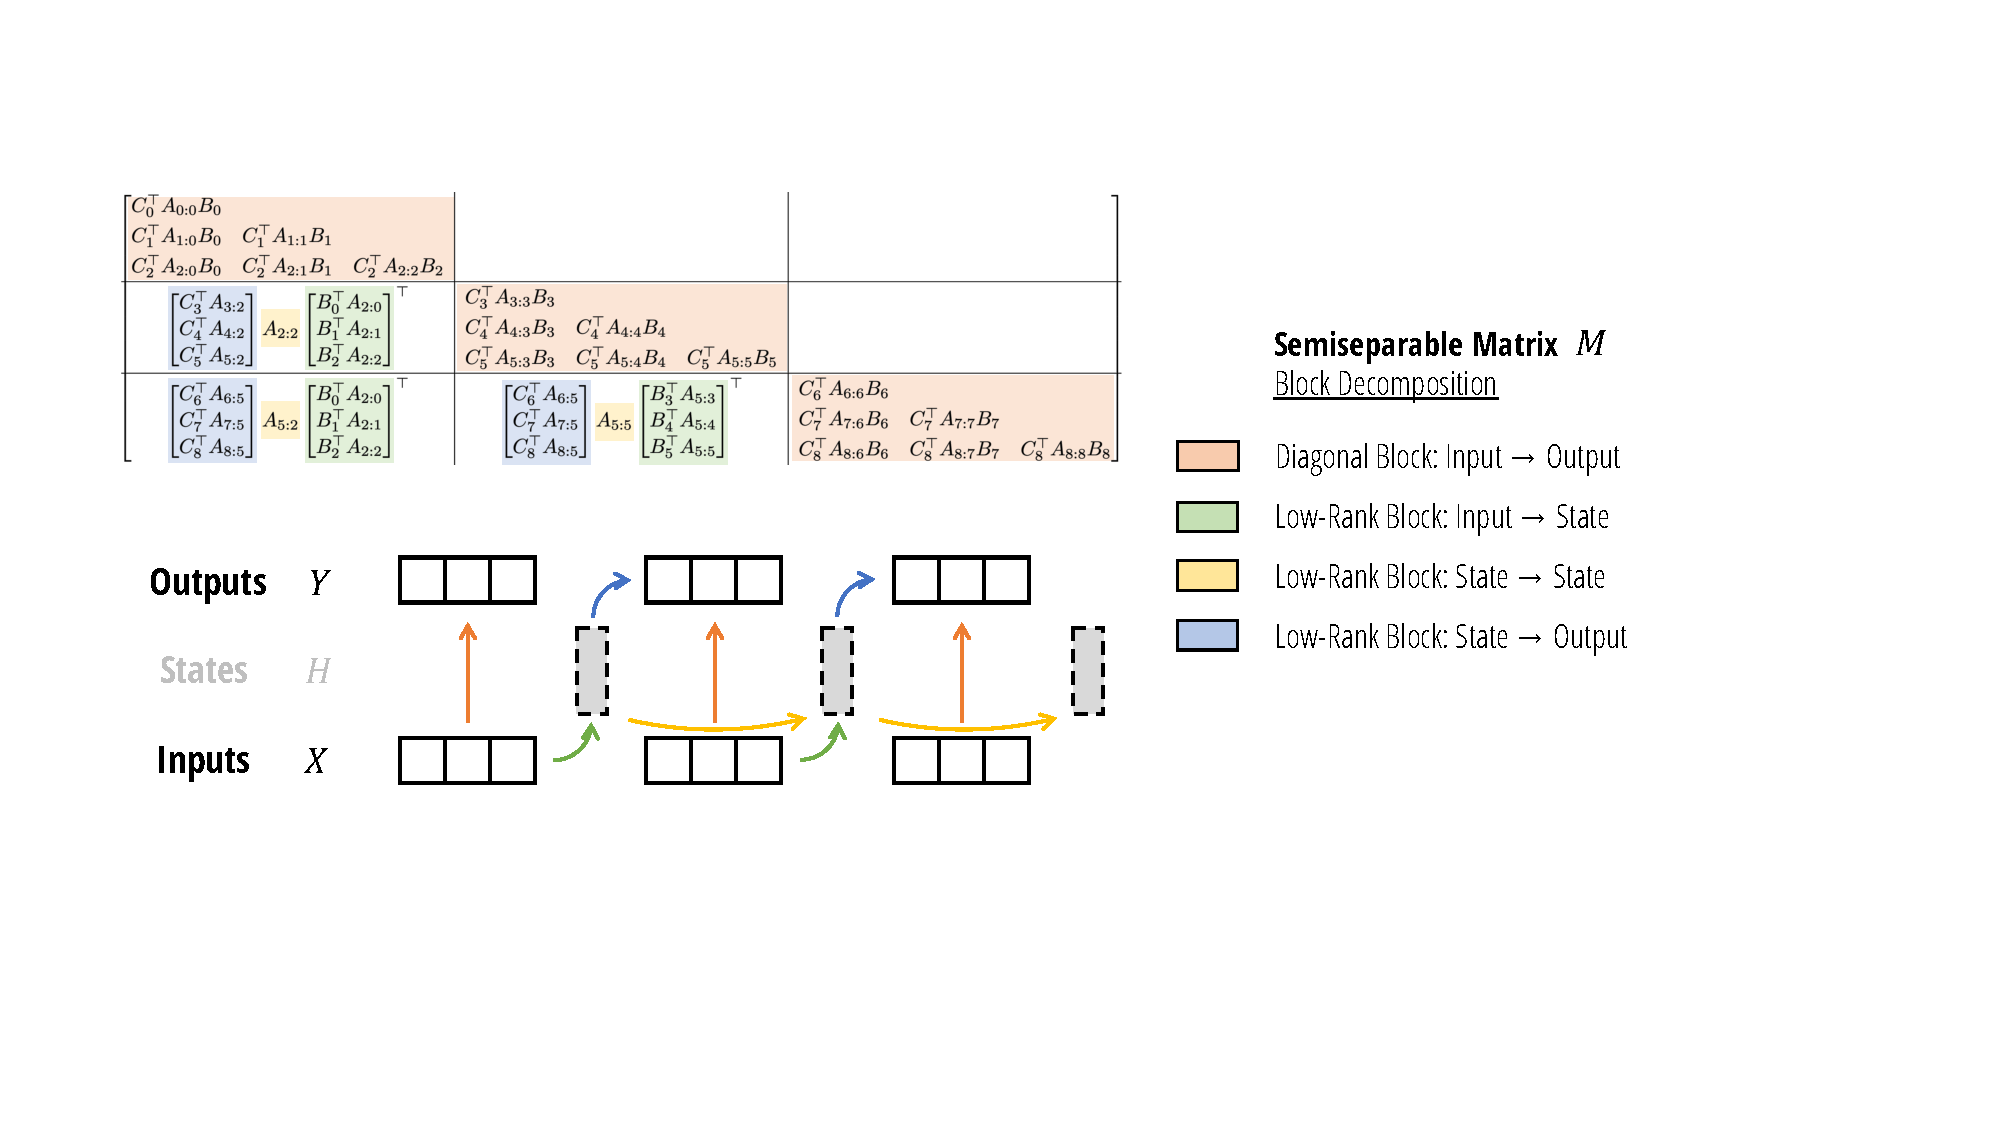
\includegraphics[width=\linewidth]{fig/ssd_algorithm.pdf}
\caption{
  (\textbf{SSD Algorithm}.)
  By using the matrix transformation viewpoint of state space models to write them as semiseparable matrices (\cref{sec:ssm}), we develop a more hardware-efficient computation of the SSD model through a block-decomposition matrix multiplication algorithm.
  The matrix multiplication also has an interpretation as a state space model,
  where blocks represent chunking the input and output sequence.
  Diagonal blocks represent intra-chunk computations and the off-diagonal blocks represent inter-chunk computations, factored through the SSM's hidden state.
}
\label{fig:ssd-algorithm}
\end{figure}

\subsection{Computational Cost}

We define the notation $\mathsf{BMM}(\mathtt{B}, \mathtt{M}, \mathtt{N}, \mathtt{K})$ to define a batched matrix multiplication $\mathsf{contract}(\mathtt{\mathtt{MK},\mathtt{KN} \to \mathtt{MN}})$ with batch dimension $\mathtt{B}$.
From this notation we can infer three aspects of the efficiency:
\begin{itemize}
  \item \emph{Computation cost}: total of $O(\mathtt{BMNK})$ FLOPs.
  \item \emph{Memory cost:} total of $O(\mathtt{B}(\mathtt{MK}+\mathtt{KN}+\mathtt{MN}))$ space.
  \item \emph{Parallelization:} larger $\mathtt{M}, \mathtt{N}, \mathtt{K}$ terms can leverage specialized matrix multiplication units on modern accelerators.
\end{itemize}

\paragraph{Center Blocks.}
The cost of the quadratic SMA computation consists of three steps (equation \eqref{eq:ssm-quad}):
\begin{itemize}
  \item Computing the kernel matrix $C^{\top} B$, which has cost $\mathsf{BMM}(\mathtt{T}/\mathtt{Q}, \mathtt{Q}, \mathtt{Q}, \mathtt{N})$.
  \item Multiplying by the mask matrix, which is an elementwise operation on tensors of shape $(\mathtt{T}/\mathtt{Q}, \mathtt{Q}, \mathtt{Q})$.
  \item Multiplying by the $X$ values, which has cost $\mathsf{BMM}(\mathtt{T}/\mathtt{Q}, \mathtt{Q}, \mathtt{P}, \mathtt{N})$
\end{itemize}

\paragraph{Low-Rank Blocks: Right Factors.}
This step is a single matrix multiplication with cost $\mathsf{BMM}(\mathtt{T}/\mathtt{Q}, \mathtt{N}, \mathtt{P}, \mathtt{Q})$.

\paragraph{Low-Rank Blocks: Center Factors.}
This step is a scalar SSM scan (or 1-SS multiplication) of length $\mathtt{T}/\mathtt{Q}$ on $(\mathtt{N}, \mathtt{P})$ independent channels.
The work of this scan is $\mathtt{TNP}/\mathtt{Q}$, which is negligible compared to the other factors.

Note that because of the blocking which reduces the length of the sequence from $\mathtt{T}$ to $\mathtt{T}/\mathtt{Q}$,
this scan has $\mathtt{Q}$ times smaller cost than a pure SSM scan (e.g. the selective scan of Mamba).
Thus we observe that on most problem lengths,
other algorithms (\cref{sec:scan}) may be more efficient or much easier to implement without a significant slowdown.
For example, a naive implementation of this via 1-SS matrix multiplication has cost $\mathsf{BMM}(1, \mathtt{T}/\mathtt{Q}, \mathtt{NP}, \mathtt{T}/\mathtt{Q})$,
which is much easier to implement and can be more efficient than a naive recurrence/scan implementation.

\paragraph{Low-Rank Blocks: Left Factors.}
This step is a single matrix multiplication with cost $\mathsf{BMM}(\mathtt{T}/\mathtt{Q}, \mathtt{Q}, \mathtt{P}, \mathtt{N})$.

\paragraph{Total Cost.}
If we set $\mathtt{N} = \mathtt{P} = \mathtt{Q}$ (in other words the state dimension, head dimension, and chunk length are equal),
then all BMM terms above become $\mathsf{BMM}(\mathtt{T}/\mathtt{N}, \mathtt{N}, \mathtt{N}, \mathtt{N})$.
The computational chacteristics of this are:
\begin{itemize}
  \item Total FLOP count of $O(\mathtt{TN}^2)$.
  \item Total memory of $O(\mathtt{TN})$.
  \item The work \emph{consists primarily of matrix multiplications} on matrices of shape $(\mathtt{N}, \mathtt{N})$.
\end{itemize}
Notice that the memory consumption is tight; the inputs and outputs $x, y$ have shape $(\mathtt{T}, \mathtt{P}) = (\mathtt{T}, \mathtt{N})$.
Meanwhile the flop count reflects an extra factor of $\mathtt{N}$, which is cost incurred by the autoregressive state size and is common to all models.

Aside from the matmuls, there is a scalar SSM scan on $\mathtt{NP} = \mathtt{N}^2$ features and sequence length $\mathtt{T}/\mathtt{Q}$.
This has cost $O(\mathtt{T}/\mathtt{Q} \mathtt{N}^2)$ FLOPs and $O(\log(\mathtt{T}/\mathtt{Q}))$ depth.
Although it does not use matrix multiplications, it is still parallelizable and the total work done is negligible compared to the other steps;
this has a negligible cost in our GPU implementation.

\paragraph{Comparison to Pure SSM and Attention Models.}

Quadratic attention is also very hardware efficient by only leveraging matrix multiplications, but has $\mathtt{T}^2 N$ total FLOPs.
Its slower computation speed at both training and inference can directly be seen as a consequence of having a larger state size -- standard attention has a state size scaling with sequence length $\mathtt{T}$ because it caches its history and does not compress its state.

Linear SSMs have $\mathtt{TNP} = \mathtt{TN}^2$ total FLOPs, which is the same as SSD.
However, a naive implementation requires a state expansion \eqref{eq:sha-lin:1} that materializes extra memory,
and a scalar operation \eqref{eq:sha-lin:2} that does not leverage matrix multiplications.


\begin{center}
  \begin{tabular}{@{}llll@{}}
    \toprule
                            & Attention                & SSM                                        & \textbf{SSD} \\
    \midrule
    State size              & $\mathtt{T}$             & $\mathtt{\mathbf{N}}$                      & $\mathtt{\mathbf{N}}$ \\
    Training FLOPs          & $\mathtt{T}^2\mathtt{N}$ & $\mathtt{\mathbf{T}}\mathtt{\mathbf{N}}^2$ & $\mathtt{\mathbf{T}}\mathtt{\mathbf{N}}^2$ \\
    Inference FLOPs         & $\mathtt{T}\mathtt{N}$   & $\mathtt{\mathbf{N}}^2$                    & $\mathtt{\mathbf{N}}^2$ \\
    \midrule
    (Naive) memory          & $\mathtt{T}^2$           & $\mathtt{T}\mathtt{N}^2$                   & $\mathtt{\mathbf{T}}\mathtt{\mathbf{N}}$ \\
    Matrix multiplication   & \cmark                   &                                            & \textbf{\cmark} \\
    \bottomrule
  \end{tabular}
  \label{tab:compute}
\end{center}

We note that many other matrix decompositions are possible (for example, see \cref{sec:scan} for a compendium of algorithms for 1-SS multiplication through different structured matrix decompositions)
which may lead to more algorithms for SSDs that could be better for other specialized settings.
Even more broadly, we note that semiseparable matrices have a rich literature and many more representations besides the SSS form that we use (\cref{def:sss}),
and even more efficient algorithms may be possible.
